%\setchapterimage{fig_00.jpg}
\chapter*{Application \arabic{cptApplication} \\ 
Machines Synchrones -- Alternateur
-- \ifprof Corrigé \else Sujet \fi}
\addcontentsline{toc}{section}{Application \arabic{cptApplication} : 
Machines Synchrones -- Alternateur
-- \ifprof Corrigé \else Sujet \fi}

\iflivret \stepcounter{cptApplication} \else
\ifprof  \stepcounter{cptApplication} \else \fi
\fi

\setcounter{question}{0}
\marginnote{Ressources de Philippe Dubois.}


La plaque signalétique d'un alternateur\sidenote{Est-ce vraiment un alternateur ? Est-il vraiment utilisé en tant que tel ?} triphasé donne : 
\begin{itemize}
\item $S =\SI{2}{MVA}$; 
\item $\SI{2885}{V}/\SI{5000}{V}$;
\item $\SI{50}{Hz}$ ;
\item $\SI{1500}{tr/min}$.
\end{itemize}

Les enroulements sont couplés en étoile, on mesure la résistance entre deux phases $\indice{R}{mes}=\SI{0,40}{\Omega}$.
On note $L$ l'impédance d'un enroulement d'une phase.
La résistance du rotor $\indice{R}{e}=\SI{10}{\Omega}$.
L’ensemble des pertes fer et mécaniques valent $\SI{65}{kW}$.


Un essai << à vide >> donne une caractéristique d´équation $E = 100I_e$ ou $E$ est la valeur efficace de la fem induite dans un enroulement et $I_e$ est l’intensité du courant d’excitation : $0 < I_e < \SI{50}{A}$.


\question{Déterminer le nombre de pôles de la machine.}
\ifprof
\begin{marginfigure}
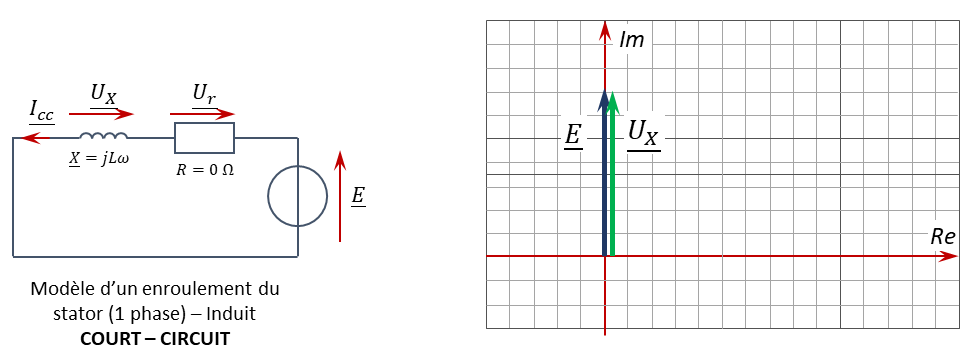
\includegraphics[width=\linewidth]{cor_01}
\end{marginfigure}

\begin{corrige}
À \si{50}{Hz} et 1 paire de pôles, on tourne à  \si{50}{tr/s} soient \si{3000}{tr/min}.  Pour aller à \si{1500}{tr/min} il faut donc 2 paires de pôles. 

On a aussi $N_s = \dfrac{60f}{p}$ $\Rightarrow p =\dfrac{60\times 50}{1500} = 2$.
\end{corrige}
\else
\fi

\question{Rappeler dans quelles conditions est réalisé l'essai << à vide >>.} 
\ifprof
\begin{corrige}
Source ? Moteur entrainé par un MCC à la vitesse de synchronisme ? On mesure une tension simple sur le stator ? et le courant dans le rotor ? LE courant dans le moteur s'appelle courant d'excitation ? On fait comment pour le mesurer ?

\end{corrige}
\else
\fi

\question{Déterminer la résistance $r$ d'un enroulement statorique.}
\ifprof
\begin{marginfigure}
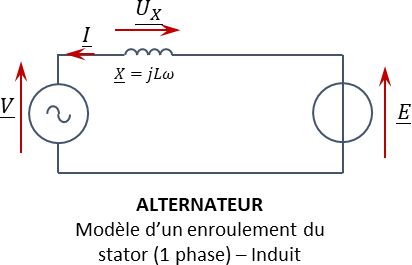
\includegraphics[width=\linewidth]{cor_02}
\end{marginfigure}

\begin{marginfigure}
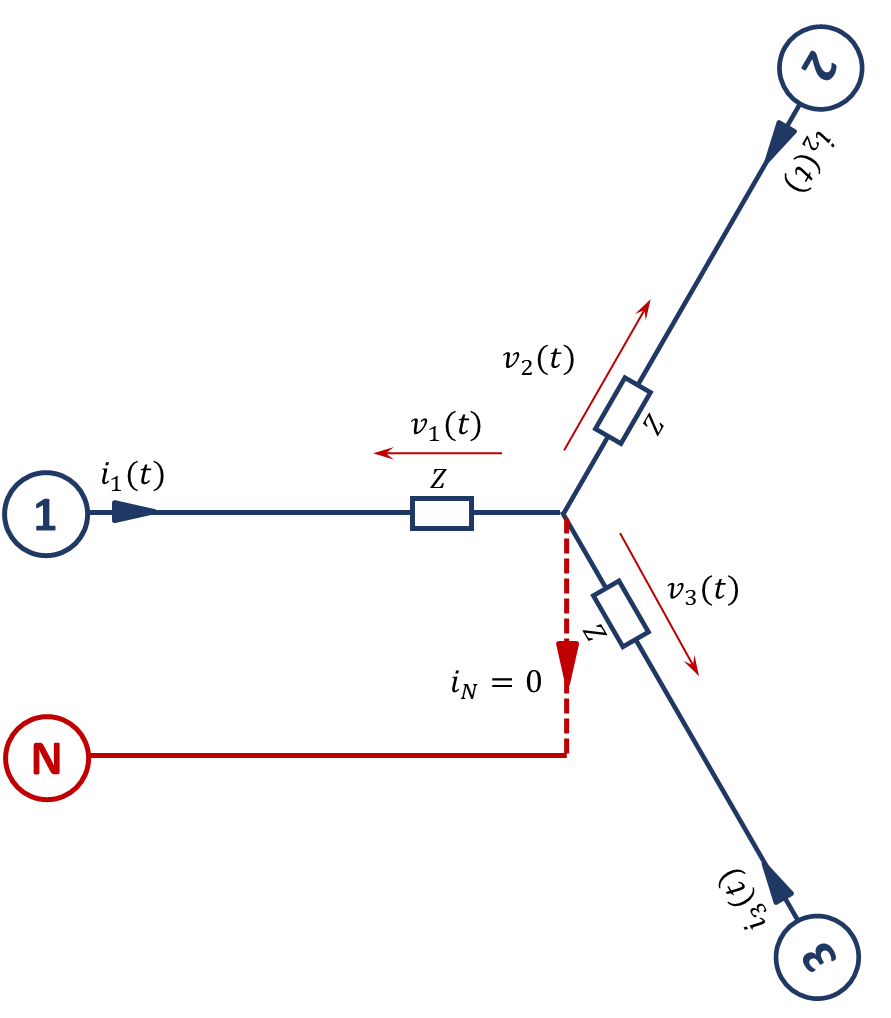
\includegraphics[width=\linewidth]{cor_03}
\end{marginfigure}

\begin{corrige}
Il s'agit ici d'un couplage en étoile. On mesure la résistance entre deux phases. Dans cette configuration, on mesure la tension aux bornes de deux enroulements en série. En notant $r$ la résistance d'un enroulement, on a donc $\indice{R}{mes}=2r$.

\textit{AN :} $r = \SI{0,2}{\Omega}$.

\end{corrige}
\else
\fi



\question{Donner le schéma équivalent d’un enroulement.}
\ifprof
\begin{corrige}
\begin{center}
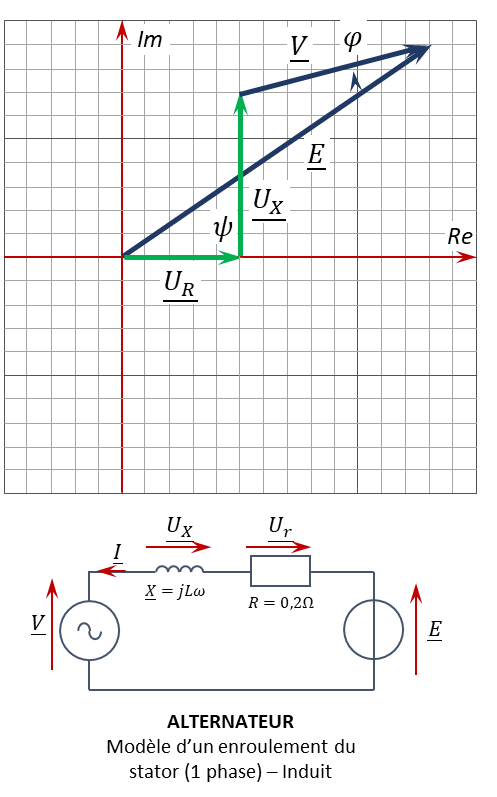
\includegraphics[width=.5\linewidth]{cor_04}
\end{center}
\end{corrige}
\else
\fi



En charge cet alternateur alimente une installation triphasée équilibrée, inductive, de facteur puissance 0,80, sous une tension efficace nominale $U_n = \SI{5000}{V}$ entre phases \sidenote{Piege ? Indication à virer sachant qu'après on a besoin de la tension simple et pas de la tension composée ?}. 
L’intensité efficace du courant en ligne est alors $I_n = \SI{200}{A}$ et le courant d´excitation $I_e = \SI{32}{A}$.

%Traiter les questions suivantes pour un fonctionnement << en charge >>.

\question{Tracer le diagramme de Fresnel.}
\ifprof
\begin{marginfigure}
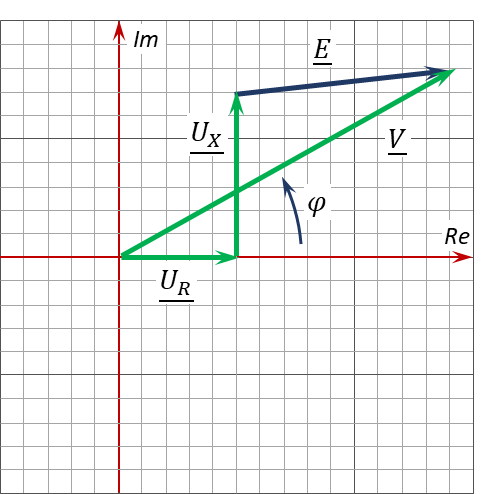
\includegraphics[width=\linewidth]{cor_05}
\end{marginfigure}
\begin{corrige}
La loi des mailles en notation complexe s'écrit 
$\underline{V} = \underline{U_X} + \underline{U_r} + \underline{E}$. 
Par ailleurs, 
$\underline{I} = I_n \sqrt{2}$, 
$\underline{E} = 100I_e \sqrt{2}e^{j\psi}$, 
$\underline{V} = Ve^{j\varphi}$ tel que $\cos\varphi = 0,8$ et $V = \indice{V}{eff} \sqrt{2}= 2885 \sqrt{2}$, 
$\underline{U_r} = R\underline{I} $ et 
$\underline{U_X} = j L \omega \underline{I}$.
\end{corrige}
\else
\fi

\question{En faisant l'hypothèse que $r<< L \omega_s$, déterminer la valeur de $L$.}
\ifprof
\begin{corrige}
La loi des mailles devient $\underline{V} = \underline{U_X} +  \underline{E}$.
On a alors 
$\left\{
\begin{array}{l}
E\cos \psi = \indice{V}{eff} \sqrt{2} \cos\varphi \\
E\sin \psi + L\omega I_n \sqrt{2} = \indice{V}{eff} \sqrt{2}\sin\varphi \\
\end{array}
\right.
$
soit 
$\left\{
\begin{array}{l}
E\cos \psi = \indice{V}{eff} \sqrt{2} \cos\varphi \\
E\sin \psi = \indice{V}{eff} \sqrt{2}\sin\varphi -  L\omega I_n \sqrt{2}\\
\end{array}
\right.
$.
On a donc 
$2 \times 100^2 I_e^2  = 2\indice{V}{eff}^2 \cos^2\varphi +  2 \indice{V}{eff}^2 \sin^2\varphi + 2L^2\omega^2 I_n^2 - 
4 \indice{V}{eff} I_n  L \sin\varphi $

$\Rightarrow   100^2 I_e^2  = \indice{V}{eff}^2 + L^2\omega^2 I_n^2 - 2 \indice{V}{eff} I_n  L\omega \sin\varphi $

$\Rightarrow    L^2\omega^2 I_n^2 - 2 \indice{V}{eff} I_n  L\omega \sin\varphi + \indice{V}{eff}^2 - 100^2 I_e^2  = 0 $

Résolution d'un polynôme d'ordre 2 : $L\omega = \SI{19,7}{\Omega}$.
\end{corrige}
\else
\fi

\question{Calculer la puissance utile, les différentes pertes, la puissance absorbée totale, le rendement et le moment du couple nécessaire pour entrainer la machine synchrone.}
\ifprof
\begin{corrige}

\begin{itemize}
\item La puissance active (qui est donc utile ?) reçue par les 3 enroulements est $P_u = 3 \indice{V}{eff}\indice{I}{eff} \cos \varphi$ ($\indice{I}{eff}=I_n$). \textit{AN} : $P_u = 3 \times 2885 \times 200 \times 0,8 =\SI{1384,8}{kW} $. (On pourrait aussi utiliser la tension composée $P_u = 3 \dfrac{\indice{U}{eff}}{\sqrt{3}}\indice{I}{eff} \cos \varphi = \sqrt{3}\indice{U}{eff}\indice{I}{eff} \cos \varphi$).
\item Pertes et fer et pertes mécaniques : $\indice{P}{fm}= \SI{65}{kW}$.
\item Pertes effet Joule stator : $\indice{P}{Js} = 3 r I_n^2$. \textit{AN} : $P_j = 3 \times 0,2 \times 200^2 =\SI{24}{kW}$.
\begin{itemize}
\item Puissance des pertes totales $P_p =\indice{P}{fm}+\indice{P}{Js} =\SI{89}{kW}$. 
\end{itemize}
\end{itemize}

La puissance absorbée (c'est quoi en fait ?) $\indice{P}{em} = P_u-P_p=\SI{1295,8}{kW}$.

Le couple mécanique est donc $C = \dfrac{\indice{P}{em}}{1500\times2 \times \pi / 60} = \SI{8,2}{kN.m} $.

Rendement : $\eta = \dfrac{\indice{P}{em}}{P_u}= \SI{93}{\%}$.
\end{corrige}
\else
\fi

\ifprof
\else
\begin{marginfigure}[-3cm]
\centering
%\includegraphics[width=3cm]{Cy_02_Ch_01_Activation_01_qr}
\end{marginfigure}
\fi




